\section{General architecture}
The goal of this project is to allow for applications to modify files stored in different locations through the Ubuntu One protocols.\\

In order to achieve this, several components are necesary:
\begin{itemize}
\renewcommand{\labelitemi}{$\bullet$}
   \item The server: It receives instructions through the Ubuntu One API over HTTP.
   \item The clients: They are the user side. Those clients exchange with the server over the API.
   \item The \textit{drivers} : The \textit{drivers} enable the server to comunicate with the different storing facilities.
\end{itemize}

\begin{figure}
    \center
    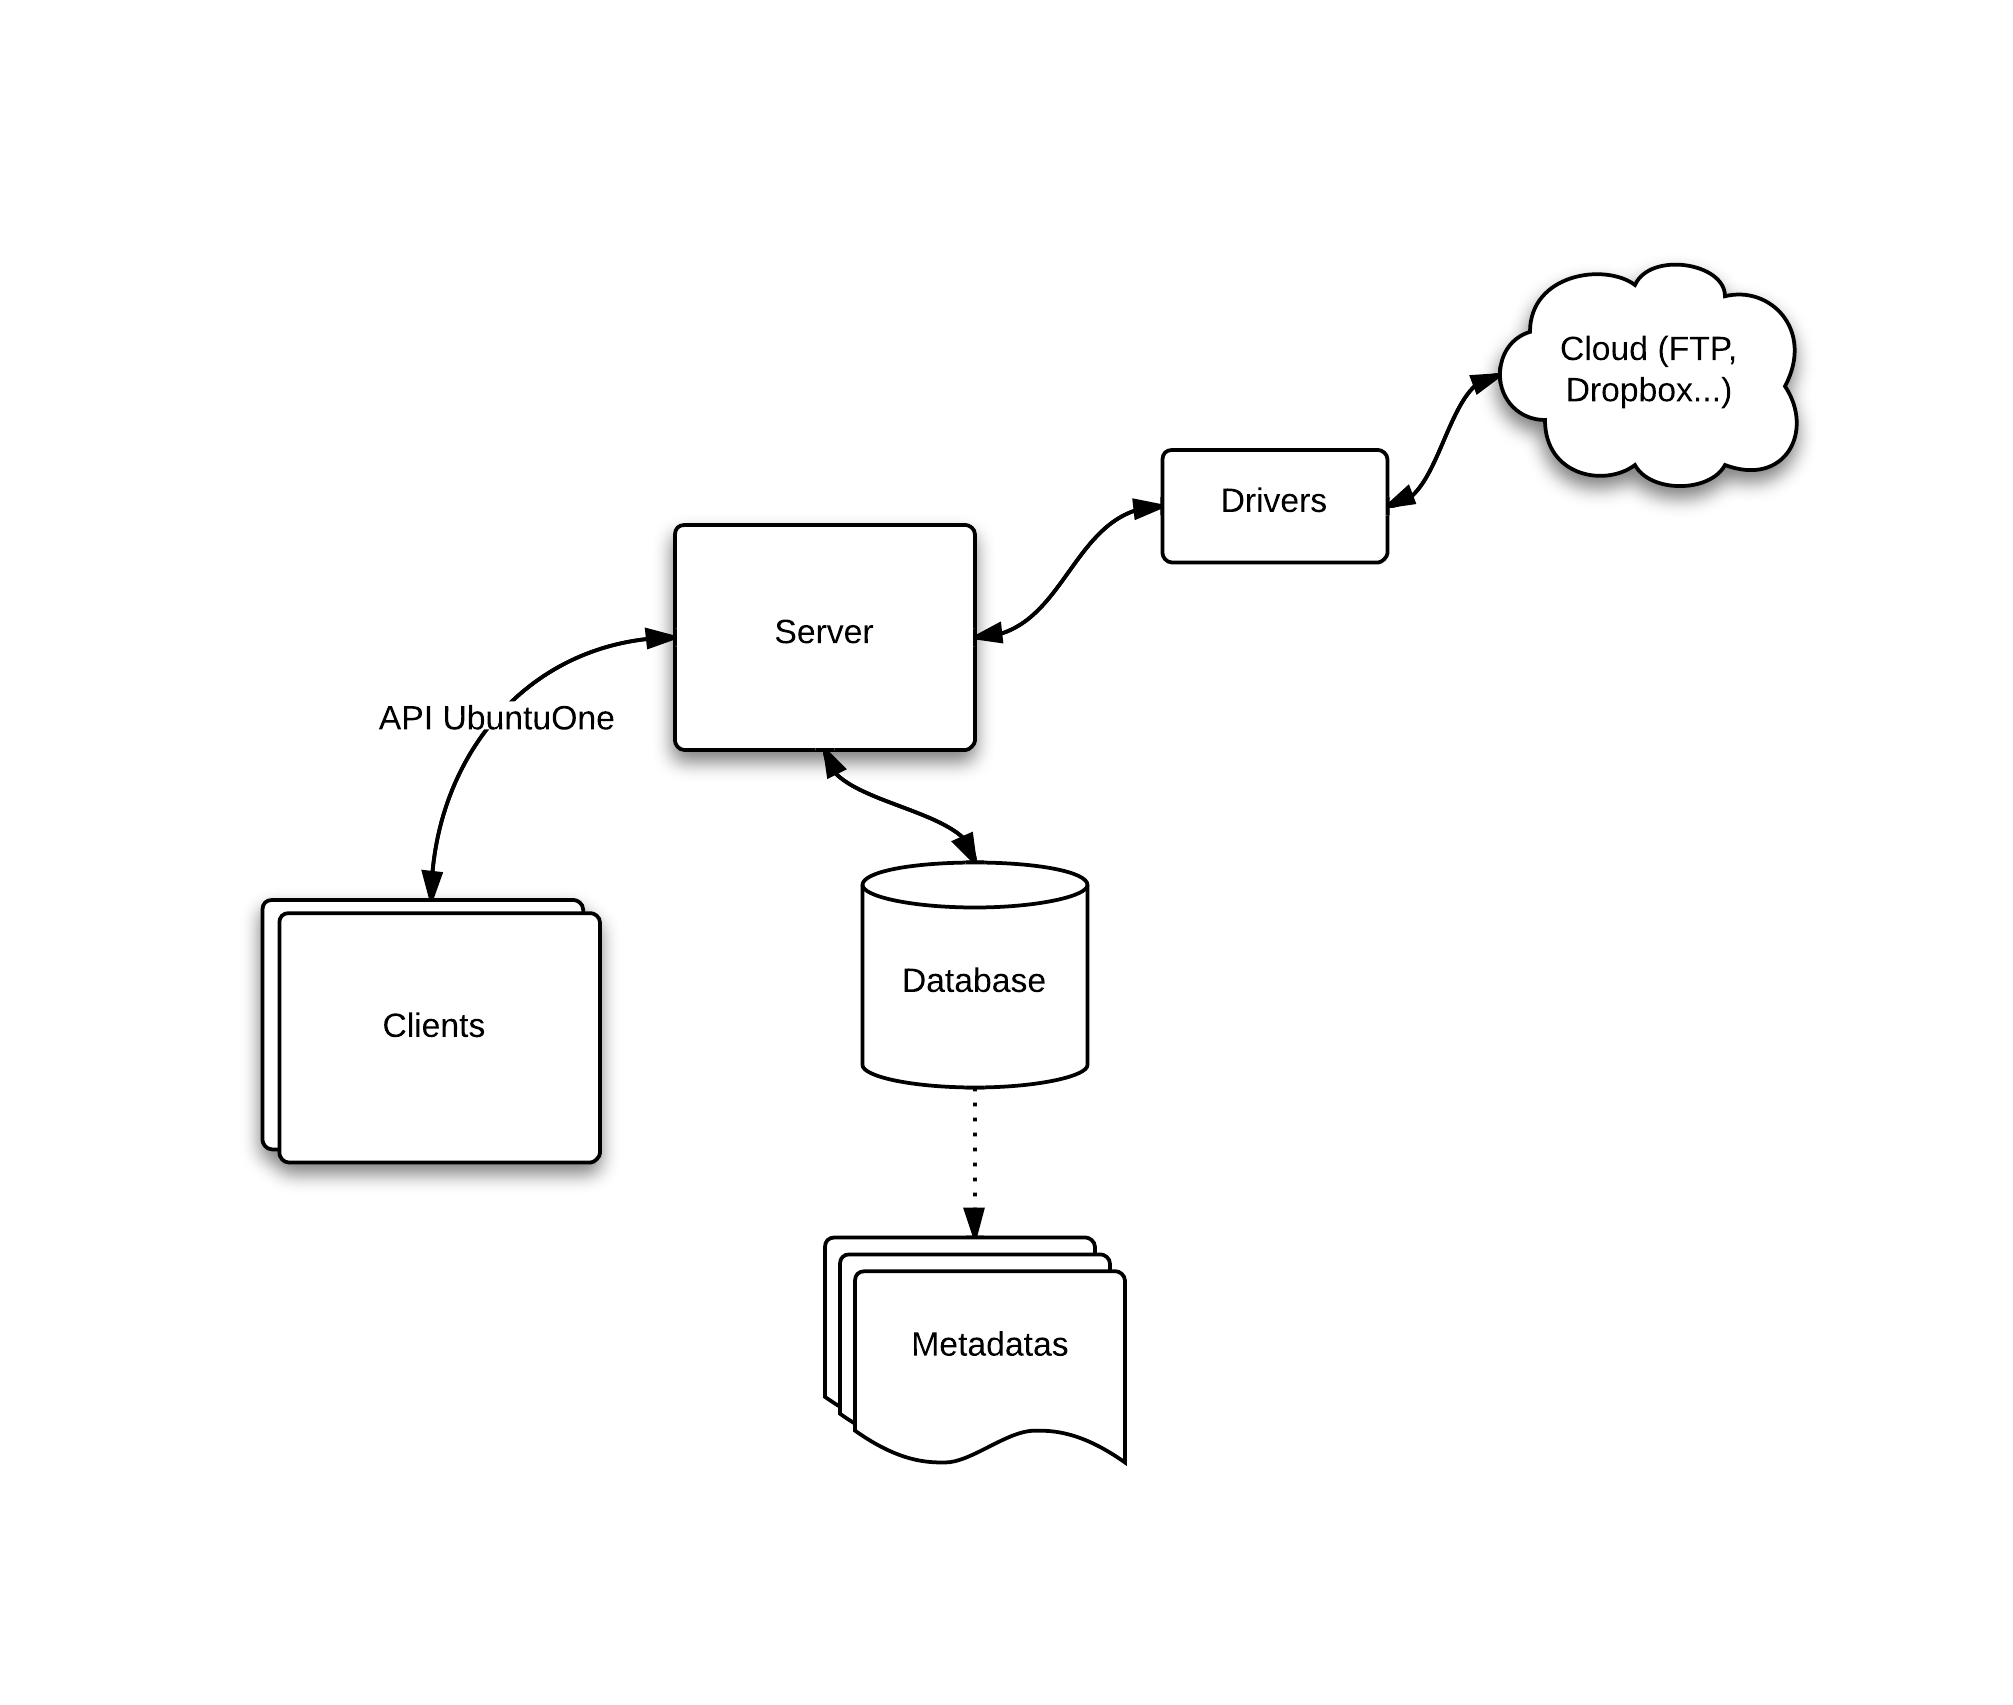
\includegraphics[width=500pt]{architecture.png}
    \caption{General project architecture.}
\end{figure}

\section{Server}
The server is the central part of the project. It must understand the instructions sent by the clients and handle them.\\

One implementation has been done by the compagny Canoncical, which is behind Ubuntu One. This implementation uses the services of Cloud Computing EC2 and Amazon's S3. Because of an agreement between those two compagnies the source code of the Ubuntu One server isn't available and will \textit{probably} never be.\\

Onitu enables its users to choose between several storage solutions for their data. From the server's point of view this is possible because of meta-data stored in a database which containes the necesary informations for \textit{drivers} to retrieve the requested information.\\

\section{Drivers}
The \textit{drivers} allow comunication between the server and the different storage facilities. They are build around a common interface that they extend in orfer to interact with the backend they are designed for.\\

All th e\textit{drivers} must allow the four basic opperations: Creation of a file, its retrieval, its edition and its deletion. (This is known under the acronym \textit{CRUD}, which stands for \textit{Create, Read, Update, Delete}).\\

Because Onitu is open source software, anyone can built its own \textit{driver}, but several are planned and will be maintained in the scope of this EIP:
\begin{itemize}
\renewcommand{\labelitemi}{$\bullet$}
    \item \textbf{Local storage} : Backed by the filesystem, this allows storage on the server where Onitu is instaleld.
    \item \textbf{Dropbox/Box.com/Google Drive/SkyDrive} : Onitu can also use those external services to retrieve and store files if the users has access to them.
    \item \textbf{(S)FTP/SSH/NFS/Webdav/Samba/HTTP} : Those drivers are backed by standart protocols, and allow to interact with other servers which at least understands one of them. This allows for easy extention of the storage whitout depending on some service he doesnt master.
    \item \textbf{Amazon S3} : Onitu can use Amazon's cloud storage, which is among the most used storage services in the world.
    \item \textbf{OwnCloud} : OwnCloud is similar service to Onitu, which makes it interesting to use them together.
    \item \textbf{Ubuntu One} : It is also possible to link other Ubuntu-One compatible servers as data storage. This means another instance of Onitu or the official Canonical server.
\end{itemize}

\section{Database}
The meta-data linked to the files will be stored in a database on the server. The major part of those metadatas are defined by the Ubuntu One protocol.\\

Onitu extends those meta-data by adding information needed by the \textit{drivers}. The exact content of thos informations are left to each \textit{driver} implementation to decide.\\

This flexibility is possibile thanks to the use of NoSQL, documente-oriented database: MongoDB.

\section{Clients}
Clients already exist for Ubuntu One on a great number of platforms plateformes (Linux, Windows, Mac OS, Android, iOS). Onitu beeing entirely compatible with Ubuntu One's API, thos clients can interact with it.\\

However, most of the clients do not currently allow the user to specify the server's address because the only existing server ts the offcial one. It is expected we will be able to integrate a way to change this address in the different clients.\\

Onitu's goal is not to provide clients bu a server. Clients may however be developed by the team for testing purposes, or to provide more usefull features to its users. A client using \textit{FUSE}, a library to create file systems, might be one of the ideas.\\

\section{Web interface}
Ubuntu One offers a web interface hosted on Amazon EC2. This interface is part of the server and its source code is not public. Onitu must procide an alternative for this web interface.

The web interface is destined to be used by the users that have the rights to access certain files and to the adminstrator who will be able to do most of the configuration through this interface.\\

The web interface has several functionalities:
\begin{itemize}
\renewcommand{\labelitemi}{$\bullet$}
    \item Load new files
    \item Edit files and file names
    \item Edit files' text easily
    \item Download files
    \item Edit file sharing rights
    \item Add, delete or edit options for the external services which are used through the drivers
    \item Edit the different options for the server's configuration
\end{itemize}
